\subsubsection{Fixed Policies across Replicated Graph Sizes}

\label{sec:scale_control}

We form one, two, four and eight disjoint copies of the clean base graph, with separate node IDs. The largest clean input has 6,984 nodes and 8,664 edges. At each size, ten fixed policy seeds and five common corruption seeds compare rate, original-count and small-count DDQN with acquire-then-deficit, giving 800 outcomes. All models were trained only at the base size. This sweep repeats the same content; it tests fixed-policy transfer rather than new documents or a large connected KG.

\begin{figure*}[t]

\centering

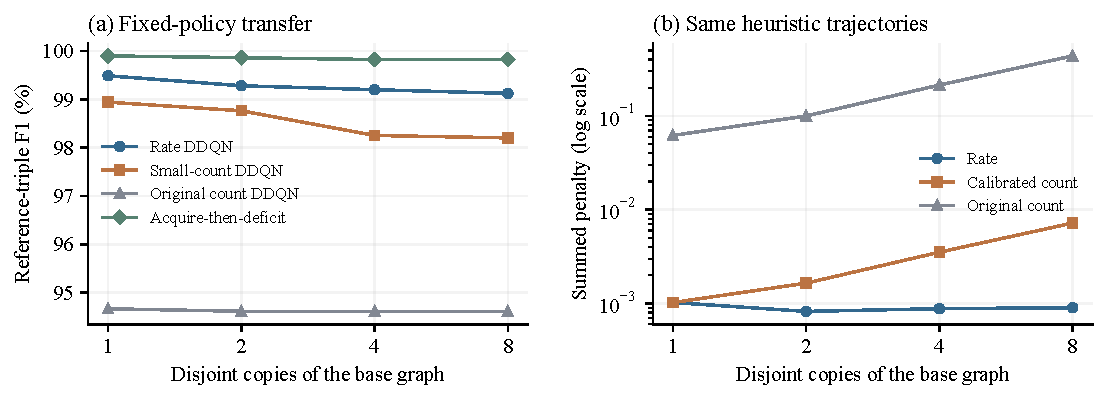
\includegraphics[width=0.94\textwidth]{figure/experiments/scale_control.pdf}

\caption{Disjoint graph-size control. (a) Mean F1 over ten model seeds and five corruption scenarios at each size. (b) Three penalties evaluated on the same heuristic trajectories. Curves are descriptive; no model is retrained or selected by size.}

\label{fig:scale_control}

\end{figure*}

\begin{table}[t]

\centering

\caption{Separate sequential heuristic resource measurement, three repeats per size. Time includes environment construction and rollout with \texttt{tracemalloc}. Memory is peak traced Python allocation, excluding the prebuilt clean graph and native tensor storage; it is not total RSS.}

\label{tab:scale_resources}

\scriptsize

\begin{tabular}{rrrr}

\toprule

Clean edges & Copies & Median seconds & Median peak MiB \\

\midrule

1,083 & 1 & 0.881 & 1.32 \\

2,166 & 2 & 1.839 & 2.89 \\

4,332 & 4 & 4.126 & 5.46 \\

8,664 & 8 & 8.805 & 11.35 \\

\bottomrule

\end{tabular}

\end{table}

On the heuristic trajectories, increasing from one to eight copies multiplies the fixed small-count burden by 7.06, compared with 0.88 for the rate burden. This measures how the penalties scale on matched behavior. Fixed-policy outcomes and same-trajectory penalties do not establish an advantage for rate-based learning across sizes; that would require training comparisons at those sizes.
